\section{Phân tích và trực quan hóa}

\subsection{Phân tích khám phá dữ liệu (EDA)}

\subsubsection{Tổng quan dữ liệu}

\textbf{Kích thước mẫu:}
\begin{itemize}
    \item Số dòng: 25,744.
    \item Số cột: 22.
    \item Kích thước bộ nhớ: 19.54 MB.
\end{itemize}

\textbf{Thống kê mô tả các biến chính:}

\begin{table}[H]
    \centering
    \caption{Thống kê mô tả các biến số đa nền tảng}
    \resizebox{\textwidth}{!}{
    \begin{tabular}{|l|c|c|c|c|c|}
        \hline
        \textbf{Biến số} & \textbf{Mean} & \textbf{Std} & \textbf{Min} & \textbf{Max} & \textbf{Median} \\
        \hline
        \multicolumn{6}{|l|}{\textbf{Chỉ số chung}} \\
        \hline
        Price / Total Cost (VND) & 2,299,920.23 & 3,482,465.02 & 1,000 & 23,261,390 & 924,750 \\
        \hline
        \multicolumn{6}{|l|}{\textbf{Chỉ số của nền tảng Tiki}} \\
        \hline
        Original Price (VND) & 537,016.06 & 1,055,922.97 & 1,000 & 6,990,000 & 195,000 \\
        \hline
        Discount Rate (\%) & 10.02 & 15.30 & 0.0 & 77.0 & 0.0 \\
        \hline
        Rating & 2.90 & 2.32 & 0.0 & 5.0 & 4.5 \\
        \hline
        Review Count & 44.07 & 213.76 & 0 & 5,490 & 1 \\
        \hline
        Sold Quantity & 696.27 & 7,657.91 & 0 & 548,705 & 13 \\
        \hline
        \multicolumn{6}{|l|}{\textbf{Chỉ số của nền tảng eBay}} \\
        \hline
        Shipping Cost (USD) & 1.29 & 4.83 & 0.0 & 30.47 & 0.0 \\
        \hline
        Seller Feedback Score & 54,858.92 & 163,401.22 & -1 & 3,329,896 & 4,757 \\
        \hline
        Seller Feedback (\%) & 96.85 & 15.02 & 0.0 & 100.0 & 99.60 \\
        \hline
    \end{tabular}
    }
    \label{tab:desc_stats}
\end{table}

\subsubsection{Phân bố các biến}




\textbf{Nhận xét:} 
Dữ liệu giá có biên độ dao động rất lớn, trải dài từ 1,000 VND đến hơn 23.2 triệu VND, đi kèm với độ lệch chuẩn cao (hơn 3.48 triệu VND) cho thấy tính phân tán mạnh. Giá trị trung bình (Mean $\approx$ 2.3 triệu VND) lớn hơn gấp đôi so với trung vị (Median $\approx$ 924 nghìn VND), minh chứng cho việc phân bố giá bị lệch phải cực mạnh. 

Nhìn sâu hơn vào các biến khác:
\begin{itemize}
    \item \textbf{Tiki:} Phân bố của \textit{Sold Quantity} và \textit{Review Count} cũng lệch phải đáng kể. Trung bình một sản phẩm bán được 696 đơn, nhưng trung vị chỉ là 13 đơn, chứng tỏ có sự chênh lệch lớn (doanh số chủ yếu đến từ một nhóm nhỏ các sản phẩm top đầu). Hơn 50\% sản phẩm trên Tiki không có hoặc có rất ít khuyến mãi (Median Discount = 0\%).
    \item \textbf{eBay:} Hầu hết người bán có mức độ uy tín rất cao (\textit{Seller Feedback \%} đạt trung vị lên tới 99.6\%). Ngoài ra, phần lớn các đơn hàng eBay trong mẫu có mức phí ship rất thấp hoặc miễn phí (Median Shipping = 0 USD), nhưng vẫn tồn tại các trường hợp phí ship lên tới hơn 30 USD tạo thành các ngoại lệ (outliers).
\end{itemize}

\subsection{Phân tích theo mục tiêu của từng thành viên}

\subsubsection{Mục tiêu 1:}



\noindent\textbf{Phương pháp trực quan:} 
    Sử dụng thống kê mô tả thông qua hai biểu đồ bổ trợ.
\begin{itemize}
    \item \textbf{Histogram:} Quan sát hình dáng phân phối và mật độ tập trung của sản phẩm theo từng phân khúc.
    \item \textbf{Boxplot:} Phân tích độ phân tán trung tâm và nhận diện trực quan biên độ của các giá trị ngoại lệ (outliers).
\end{itemize}

\vspace{0.5em}
\textbf{Kết quả trực quan hóa:}

\begin{figure}[htbp]
    \centering
    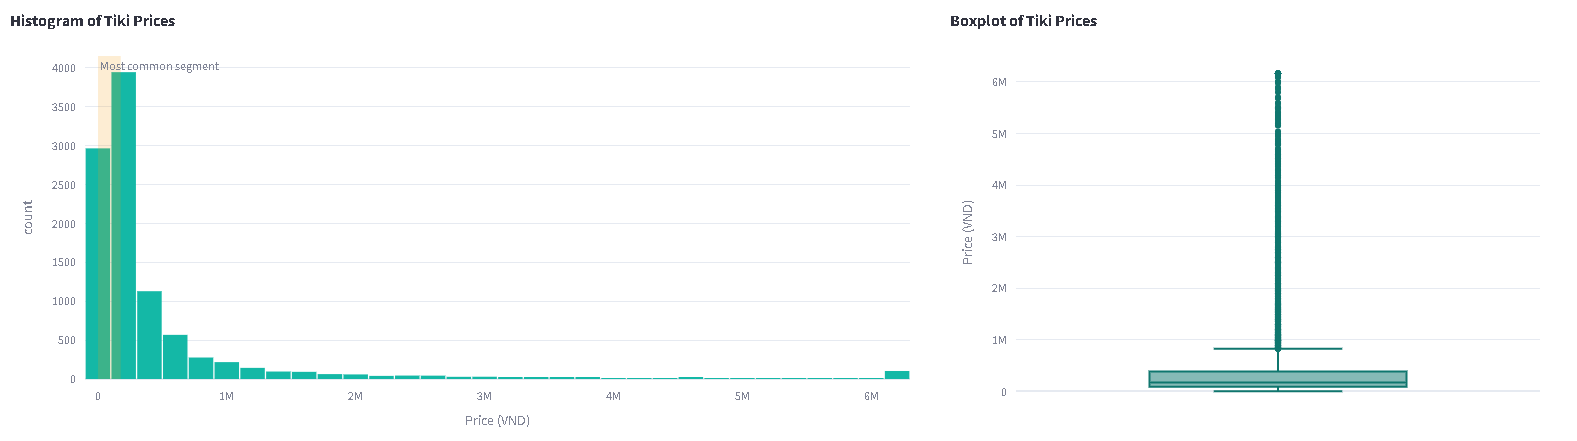
\includegraphics[width=0.95\textwidth]{graphics/tiki_price_segment_distribution.png} 
    \caption{Biểu đồ Histogram và Boxplot thể hiện phân phối mức giá sản phẩm trên nền tảng Tiki.}
    \label{fig:tiki_price_distribution}
\end{figure}

\begin{itemize}
    \item \textbf{Phân phối lệch phải cực mạnh:} Mật độ sản phẩm tập trung đông đảo nhất ở dải giá thấp. Phân khúc phổ biến nhất dao động từ \textbf{1,000 VND đến 176,994 VND}.
    \item \textbf{Boxplot nén chặt:} Khoảng tứ phân vị chứa 50\% dữ liệu cốt lõi ép rất sát trục hoành, minh chứng phần lớn mặt hàng có giá rất thấp. Kèm theo đó là dải outliers kéo dài lên tới mốc 6 triệu VND.
\end{itemize}

\vspace{0.5em}
\textbf{Nhận xét và kết luận:}
\begin{itemize}
    \item \textbf{Định vị nền tảng:} Tiki vận hành theo mô hình định giá dựa trên sản lượng, trong đó các sản phẩm bình dân là động lực tạo ra giao dịch chính.
    \item \textbf{Sự phân hóa danh mục:} Dù bị áp đảo bởi hàng giá rẻ, hàng loạt "outliers" cho thấy Tiki vẫn duy trì một ngách hàng hóa giá trị cao, tuy nhiên nhóm này không đại diện cho xu hướng chung.
    \item \textbf{Giá trị đối chiếu:} Phổ giá lệch phải của Tiki sẽ được dùng để kiểm chứng xem liệu eBay có tạo ra đường cong phân phối giá phẳng và đa dạng hơn không. Đồng thời, đánh giá xem ở phân khúc giá cao, liệu "độ uy tín gian hàng" có phải là yếu tố quyết định thay vì giá cả.
\end{itemize}

\subsubsection{Mục tiêu 2:}




\textbf{Phương pháp trực quan:} 
Sử dụng \textbf{Biểu đồ kết hợp trục kép}:
\begin{itemize}
    \item \textbf{Biểu đồ cột ghép (Trục Y trái):} So sánh số lượng Listing giữa nhóm \textit{Best Seller} và \textit{Non Best Seller}.
    \item \textbf{Biểu đồ đường (Trục Y phải):} Thể hiện xu hướng tỷ lệ mặt hàng đạt chuẩn \textit{Best Seller} theo từng phân khúc giảm giá.
\end{itemize}

\vspace{0.5em}
\textbf{Kết quả trực quan hóa:}

\begin{figure}[htbp]
    \centering
    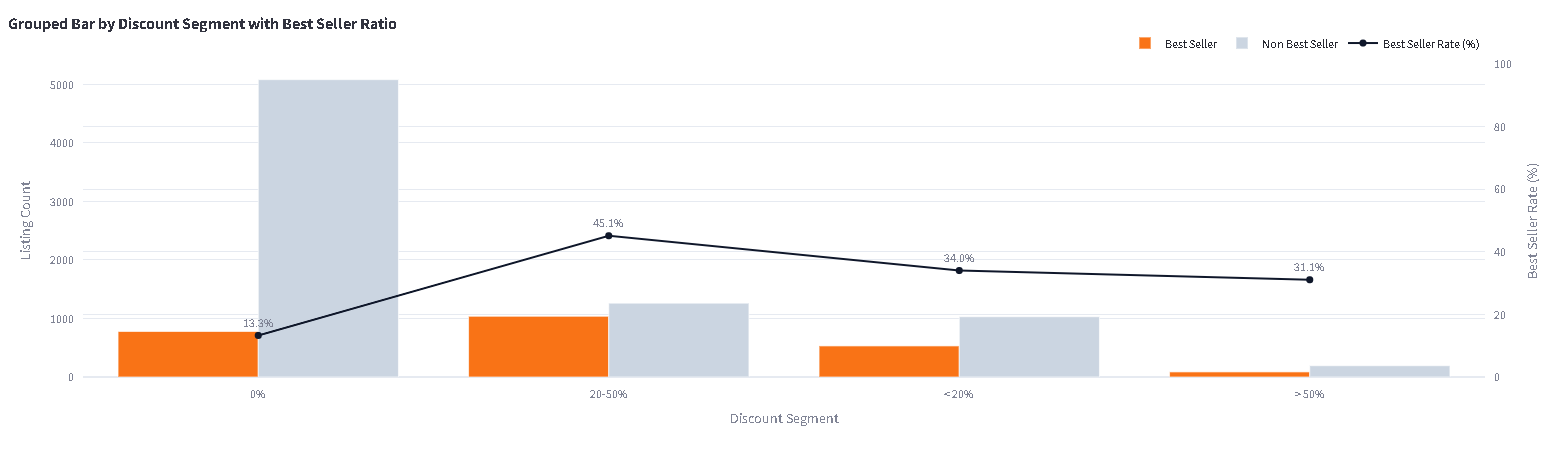
\includegraphics[width=0.95\textwidth]{graphics/tiki_focus_discount_segment_vs_best_seller.png} 
    \caption{Biểu đồ kết hợp trục kép thể hiện mức độ giảm giá và khả năng một sản phẩm trở thành Best Seller trên nền tảng Tiki..}
    \label{fig:tiki_dis_segment_vs_best_seller}
\end{figure}

\begin{itemize}
    \item \textbf{Nhóm 0\%:} Chiếm số lượng Listing áp đảo nhất nhưng tỷ lệ lọt top Best Seller lại thấp nhất, chỉ \textbf{13.3\%}.
    \item \textbf{Nhóm 20-50\%:} Ghi nhận tỷ lệ chuyển đổi thành Best Seller cao nhất, đạt đỉnh \textbf{45.1\%}.
    \item \textbf{Các nhóm khác:} Giảm nhẹ ($<$20\%) đạt mức khá (\textbf{34.0\%}); trong khi "đại hạ giá" ($>$50\%) có nguồn cung rất ít và hiệu suất giảm xuống \textbf{31.1\%}.
\end{itemize}

\vspace{0.5em}
\textbf{Nhận xét và kết luận:}
\begin{itemize}
    \item \textbf{Đặc trưng nền tảng:} Tiki là thị trường được thúc đẩy mạnh bởi khuyến mãi. Việc bán nguyên giá (0\%) tạo rào cản rất lớn trong việc chốt đơn.
    \item \textbf{"Điểm ngọt" chiến lược:} Mức chiết khấu \textbf{20\% - 50\%} là chiến lược tối ưu nhất. Giảm giá quá sâu ($>$50\%) không mang lại hiệu quả cao nhất, có thể do tạo tâm lý hoài nghi về giá trị thực của sản phẩm.
    \item \textbf{Giá trị đối chiếu:} Dữ liệu khẳng định khách hàng Tiki có tâm lý săn sale mạnh mẽ. Với bài toán đối chiếu, cần kiểm chứng xem khách hàng eBay có hành vi tương tự không, hay bị chi phối bởi yếu tố khác (mô hình đấu giá, tình trạng cũ/mới, uy tín gian hàng).
\end{itemize}



\subsubsection{Mục tiêu 3}

\textbf{Phương pháp trực quan:} 
Sử dụng biểu đồ kết hợp \textbf{Violin Plot} và \textbf{Boxplot}:
\begin{itemize}
    \item \textbf{Violin Plot:} Thể hiện mật độ phân phối của giá (Total Cost) ở các mức độ dày mỏng khác nhau, giúp nhận diện các vùng giá ``nóng'' của từng loại tình trạng.
    \item \textbf{Boxplot (nằm trong):} Cung cấp các thông số thống kê quan trọng như Trung vị (Median), Khoảng tứ phân vị (IQR) và xác định độ phân tán của giá.
\end{itemize}

\vspace{0.5em}
\textbf{Kết quả trực quan hóa:}

\begin{figure}[htbp]
    \centering
    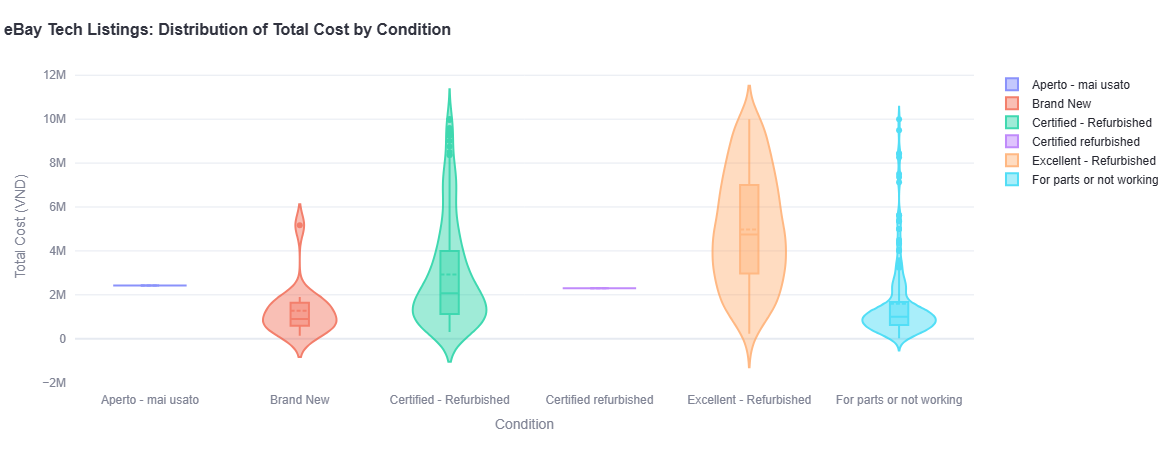
\includegraphics[width=0.95\textwidth]{graphics/ebay_price_volatility_condition.png} 
    \caption{Biểu đồ Violin và Boxplot thể hiện biến động tổng chi phí theo tình trạng hàng hóa trên eBay.}
    \label{fig:ebay_price_volatility}
\end{figure}

\begin{itemize}
    \item \textbf{Độ biến động cực lớn ở hàng Tân trang (Refurbished):} Các nhóm \textit{Certified - Refurbished} và \textit{Excellent - Refurbished} có hình dáng Violin kéo dài và rộng, với dải giá trải từ mức thấp lên đến hơn 10 triệu VND. Điều này cho thấy phân khúc hàng tân trang trên eBay rất đa dạng về chủng loại và giá trị.
    \item \textbf{Hàng Mới (Brand New) tập trung ở phân khúc thấp:} Trái với dự đoán, phần lớn hàng mới có phân phối phình to ở vùng dưới 2 triệu VND, cho thấy các mặt hàng mới trên eBay thường là linh kiện hoặc phụ kiện có giá trị nhỏ.
    \item \textbf{Nhóm hàng lấy linh kiện (For parts):} Mặc dù có giá trung vị thấp nhất, biểu đồ vẫn ghi nhận nhiều ``outliers'' lên tới mức 10 triệu VND, minh chứng cho việc các thiết bị công nghệ cao dù hỏng vẫn giữ được giá trị xác thực định đáng kể.
\end{itemize}

\vspace{0.5em}
\textbf{Nhận xét và kết luận:}
\begin{itemize}
    \item \textbf{Thế mạnh của eBay:} Biểu đồ khẳng định eBay là thị trường cực kỳ mạnh về hàng đã qua sử dụng và tân trang. Đây là nơi người dùng có thể tìm thấy nhiều lựa chọn giá trị cao (High-end) ở tình trạng không phải mới 100\%.
    \item \textbf{Sự khác biệt với Tiki:} Khác với Tiki chủ yếu bán hàng mới chính hãng, biểu đồ eBay cho thấy sự phức tạp hơn trong định giá dựa trên ``Tình trạng'' (Condition) — một yếu tố then chốt ảnh hưởng đến tâm lý quyết định mua hàng trên nền tảng quốc tế này.
\end{itemize}

\subsubsection{Mục tiêu 4}

\textbf{Phương pháp trực quan:} 
Sử dụng kết hợp hai biểu đồ bổ trợ đặt cạnh nhau:
\begin{itemize}
    \item \textbf{Biểu đồ Cột chồng (Trái):} So sánh tỷ trọng trung bình giữa Giá niêm yết (Listing Price) và Phí vận chuyển (Shipping Fee) theo từng phân khúc giá.
    \item \textbf{Biểu đồ Phân tán với đường biên (Phải):} Sử dụng đường biên $y = x$ để xác định mối quan hệ trực tiếp giữa hai loại chi phí này.
\end{itemize}

\vspace{0.5em}
\textbf{Kết quả trực quan hóa:}

\begin{figure}[htbp]
    \centering
    \begin{minipage}{0.48\textwidth}
        \centering
        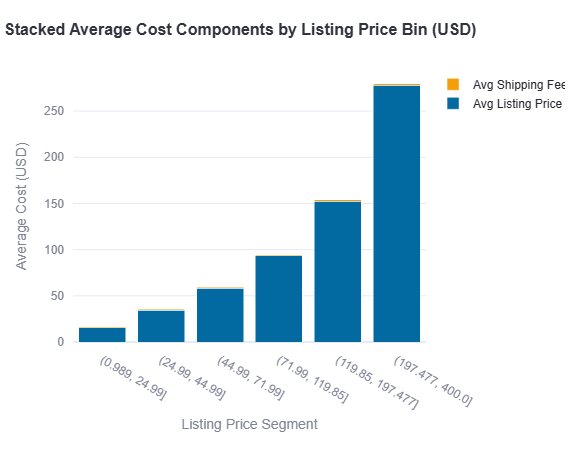
\includegraphics[width=\textwidth]{graphics/ebay_avg_cost_components.png}
        \caption{Cơ cấu chi phí theo phân khúc.}
    \end{minipage}
    \hfill
    \begin{minipage}{0.48\textwidth}
        \centering
        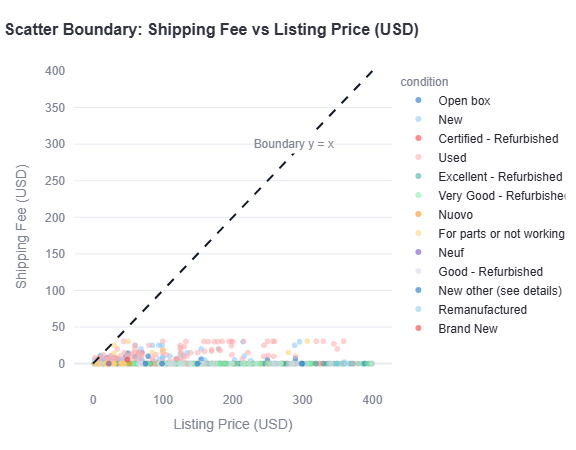
\includegraphics[width=\textwidth]{graphics/ebay_shipping_vs_listing_scatter.png}
        \caption{Tương quan phí vận chuyển và giá.}
    \end{minipage}
    \label{fig:ebay_shipping_analysis}
\end{figure}

\begin{itemize}
    \item \textbf{Phí vận chuyển chiếm tỷ trọng nhỏ:} Biểu đồ cột chồng cho thấy dù giá sản phẩm tăng từ dưới 25 USD lên đến 400 USD, phí vận chuyển trung bình vẫn giữ ở mức rất thấp (phần màu cam rất mỏng).
    \item \textbf{Ranh giới an toàn (Boundary):} Trên biểu đồ Scatter, đại đa số các điểm dữ liệu nằm sát trục hoành và cách xa đường biên $y = x$. Chỉ có \textbf{0.25\%} số lượng bản ghi có phí vận chuyển lớn hơn giá bán sản phẩm.
    \item \textbf{Tính minh bạch cao:} Hầu hết các tình trạng hàng hóa (từ New đến Used) đều tuân thủ mô hình giá sản phẩm là chi phí chủ đạo.
\end{itemize}

\vspace{0.5em}
\textbf{Nhận xét và kết luận:}
\begin{itemize}
    \item \textbf{Chiến lược người bán:} Người bán trên eBay có xu hướng không dùng phí vận chuyển để ``ngụy trang'' cho giá thực của sản phẩm. Phí vận chuyển thường được chuẩn hóa hoặc miễn phí (Free Shipping) để tăng tính cạnh tranh.
    \item \textbf{Trải nghiệm người dùng:} Với việc phí vận chuyển chỉ chiếm một phần rất nhỏ trong tổng chi phí, người mua có thể tập trung so sánh giá trị sản phẩm mà không quá lo lắng về các ``chi phí ẩn'' khi thanh toán. Điều này tạo nên một môi trường giao dịch lành mạnh và minh bạch.
\end{itemize}

\subsubsection{Mục tiêu 5}

\textbf{Phương pháp trực quan:}
\begin{itemize}
    \item \textbf{Nguyên lý Pop-out:} Sử dụng màu đỏ để nhấn mạnh 3 danh mục có rủi ro cao nhất và màu xám nhạt cho các danh mục còn lại, giúp dẫn dắt ngay sự chú ý của người xem vào trọng tâm vấn đề.
    \item \textbf{Đơn giản hóa và tối ưu Data-Ink Ratio:} Chủ động cắt bỏ phần `đuôi dài' (các danh mục có tỷ lệ tồn đọng không đáng kể) để chỉ giữ lại Top 20 trên trục hoành; đồng thời loại bỏ các đường lưới thừa nhằm giảm tải nhận thức.
    \item \textbf{Nguyên lý Connection:} Sử dụng biểu đồ đường tích lũy nối các đỉnh cột để thể hiện rõ ràng quy luật Pareto (80/20), giúp người xem dễ dàng đánh giá mức độ đóng góp dồn của các nhóm hàng đầu.
\end{itemize}

\textbf{Kết quả trực quan hóa:}

\begin{figure}[htbp]
    \centering
    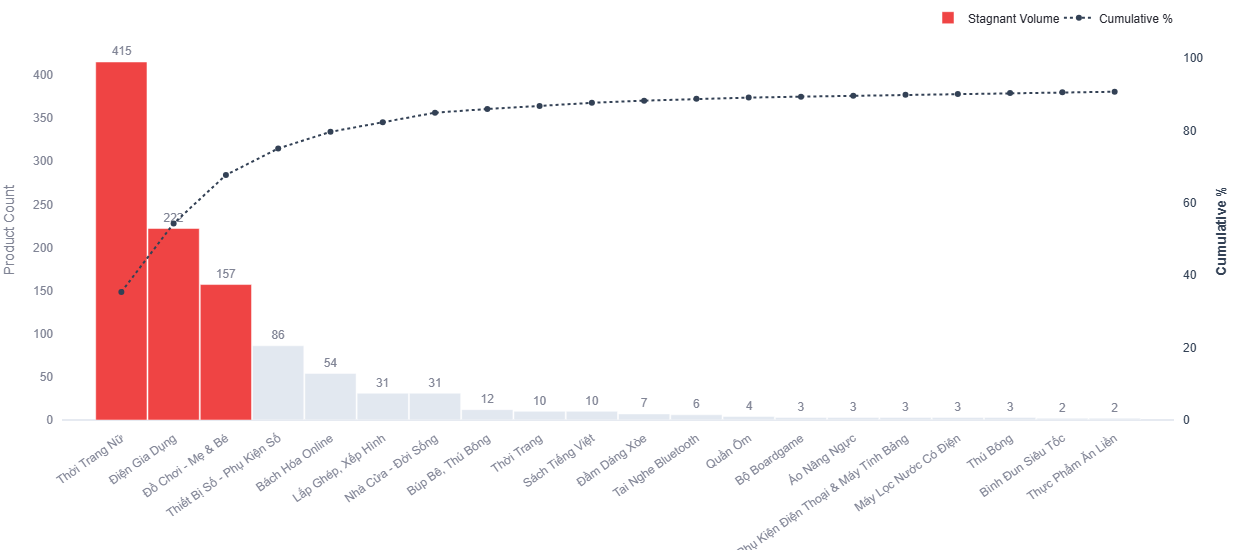
\includegraphics[width=0.85\textwidth]{graphics/tiki_pareto_coldstart.png} 
    \caption{Biểu đồ Pareto phân tích tỷ trọng sản phẩm chưa có tương tác (lượt bán và đánh giá) theo danh mục trên sàn Tiki.}
    \label{fig:tiki_pareto_coldstart}
\end{figure}

\textbf{Nhận xét và kết luận:}
\begin{itemize}
    \item Hệ thống ghi nhận có 1.173 sản phẩm (chiếm 14,5\% tổng quy mô danh mục) hoàn toàn chưa phát sinh bất kỳ giao dịch hay đánh giá nào, cho thấy một rào cản tiếp cận khách hàng tương đối lớn trên nền tảng.
    \item Tình trạng tồn đọng tuân theo quy luật Pareto: rủi ro tập trung cực độ vào 3 ngành hàng dẫn đầu là thời trang nữ (415), điện gia dụng (222) và đồ chơi - mẹ \& bé (157). Chỉ riêng 3 nhóm này đã chiếm gần 68\% tổng lượng hàng hóa chưa có giao dịch.
    \item \textbf{Kết luận:} Rủi ro tồn kho không dàn trải mà tập trung ở các ngành hàng thay đổi mẫu mã nhanh hoặc đòi hỏi độ tin cậy cao. Do đó, cần tập trung 100\% nguồn lực tiếp thị (như áp dụng Flash Sale, miễn phí vận chuyển) để xử lý cục bộ cho 3 ngành hàng trọng điểm này nhằm kích hoạt tương tác đầu tiên, thay vì phân bổ ngân sách dàn trải cho toàn bộ 14,5\% sản phẩm.
\end{itemize}

\subsubsection{Mục tiêu 6}

\textbf{Phương pháp trực quan:}
\begin{itemize}
    \item \textbf{Nguyên lý nổi bật và tương đồng:} Sử dụng đồng nhất màu xanh đậm để nhấn mạnh nhóm sản phẩm mới ở cả hai biểu đồ, kết hợp màu xám nhạt cho các nhóm còn lại. Phương pháp này giúp dẫn dắt ánh nhìn và tạo sự liên kết thông tin tự nhiên cho người xem.
    \item \textbf{Đơn giản hóa dữ liệu:} Gom nhóm dữ liệu thô từ nhiều trạng thái ngôn ngữ khác nhau thành ba nhóm trọng tâm bao gồm hàng mới, hàng đã qua sử dụng và hàng tân trang nhằm loại bỏ nhiễu thông tin và tập trung vào bức tranh tổng thể.
    \item \textbf{Tối ưu không gian hiển thị:} Sử dụng biểu đồ thanh ngang sắp xếp theo giá trị tăng dần, đồng thời loại bỏ các đường lưới và nhãn trục không cần thiết. Số liệu được ghi trực tiếp lên từng thanh ngang giúp tối ưu hóa sự tập trung và tính dễ đọc.
\end{itemize}

\textbf{Kết quả trực quan hóa:}

\begin{figure}[htbp]
    \centering
    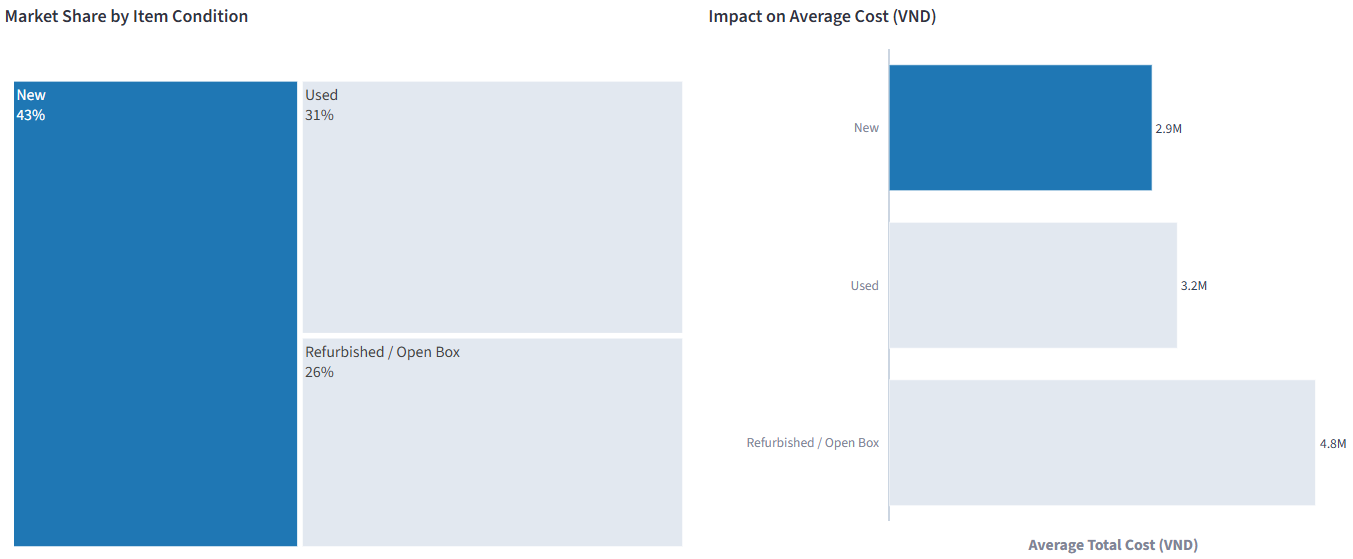
\includegraphics[width=0.95\textwidth]{graphics/ebay_condition_cost.png} 
    \caption{Biểu đồ thể hiện thị phần và chi phí trung bình theo tình trạng sản phẩm trên nền tảng eBay.}
    \label{fig:ebay_condition_cost}
\end{figure}

\textbf{Nhận xét và kết luận:}
\begin{itemize}
    \item Trong tổng số 15.528 sản phẩm hợp lệ được khảo sát, nhóm sản phẩm mới chiếm ưu thế lớn nhất với gần 43\% thị phần. Tiếp theo là nhóm hàng đã qua sử dụng chiếm 31\% và nhóm hàng tân trang chiếm 26\%.
    \item Về mặt chi phí, dữ liệu chỉ ra một xu hướng đặc biệt: nhóm sản phẩm mới lại có mức giá trung bình thấp nhất (2,9 triệu đồng), trong khi nhóm hàng tân trang lại có mức giá trị trung bình cao nhất (4,8 triệu đồng).
    \item \textbf{Kết luận:} Đặc thù giao thương trên nền tảng này cho thấy người tiêu dùng có xu hướng mua hàng mới đối với các sản phẩm thuộc phân khúc giá rẻ. Ngược lại, đối với các thiết bị có giá trị cao, họ ưu tiên lựa chọn hàng tân trang hoặc đã qua sử dụng để tối ưu chi phí. Do đó, chiến lược kinh doanh hiệu quả là tập trung bán hàng mới ở phân khúc bình dân và đẩy mạnh tìm kiếm nguồn hàng tân trang đối với phân khúc cao cấp.
\end{itemize}


\subsubsection{Mục tiêu 7}

\textbf{Phương pháp trực quan:}
\begin{itemize}
    \item \textbf{Nguyên lý Similarity (Tương đồng):} Sử dụng hệ màu sắc phân lớp (\textit{Color Ranking}) đồng nhất cho 4 mức đánh giá: Xám (Chưa có đánh giá), Đỏ (Thấp), Hổ phách (Trung bình) và Teal (Cao). Việc duy trì màu sắc này xuyên suốt các biểu đồ giúp người xem thiết lập mối liên kết tâm lý giữa màu sắc và chất lượng sản phẩm ngay lập tức.
    \item \textbf{Nguyên lý Proximity (Gần nhau):} Thiết kế biểu đồ \textit{Grouped Bar Chart} đặt các cột "Best Seller" và "Hạng thường" sát cạnh nhau trong từng nhóm Rating. Cách bố trí này cho phép so sánh trực diện hiệu quả của nhãn chứng thực lên hành vi mua hàng tại từng ngưỡng tin cậy khác nhau.
    \item \textbf{Tối ưu hóa Data-Ink Ratio:} Sử dụng biểu đồ \textit{Average Sales Bar} bổ trợ để cô đọng dữ liệu, chỉ tập trung vào việc hiển thị doanh số trung bình thay vì doanh số tổng để xác định chính xác hiệu suất thực tế của từng mức đánh giá.
\end{itemize}

\textbf{Kết quả trực quan hóa:}

\begin{figure}[htbp]
    \centering
    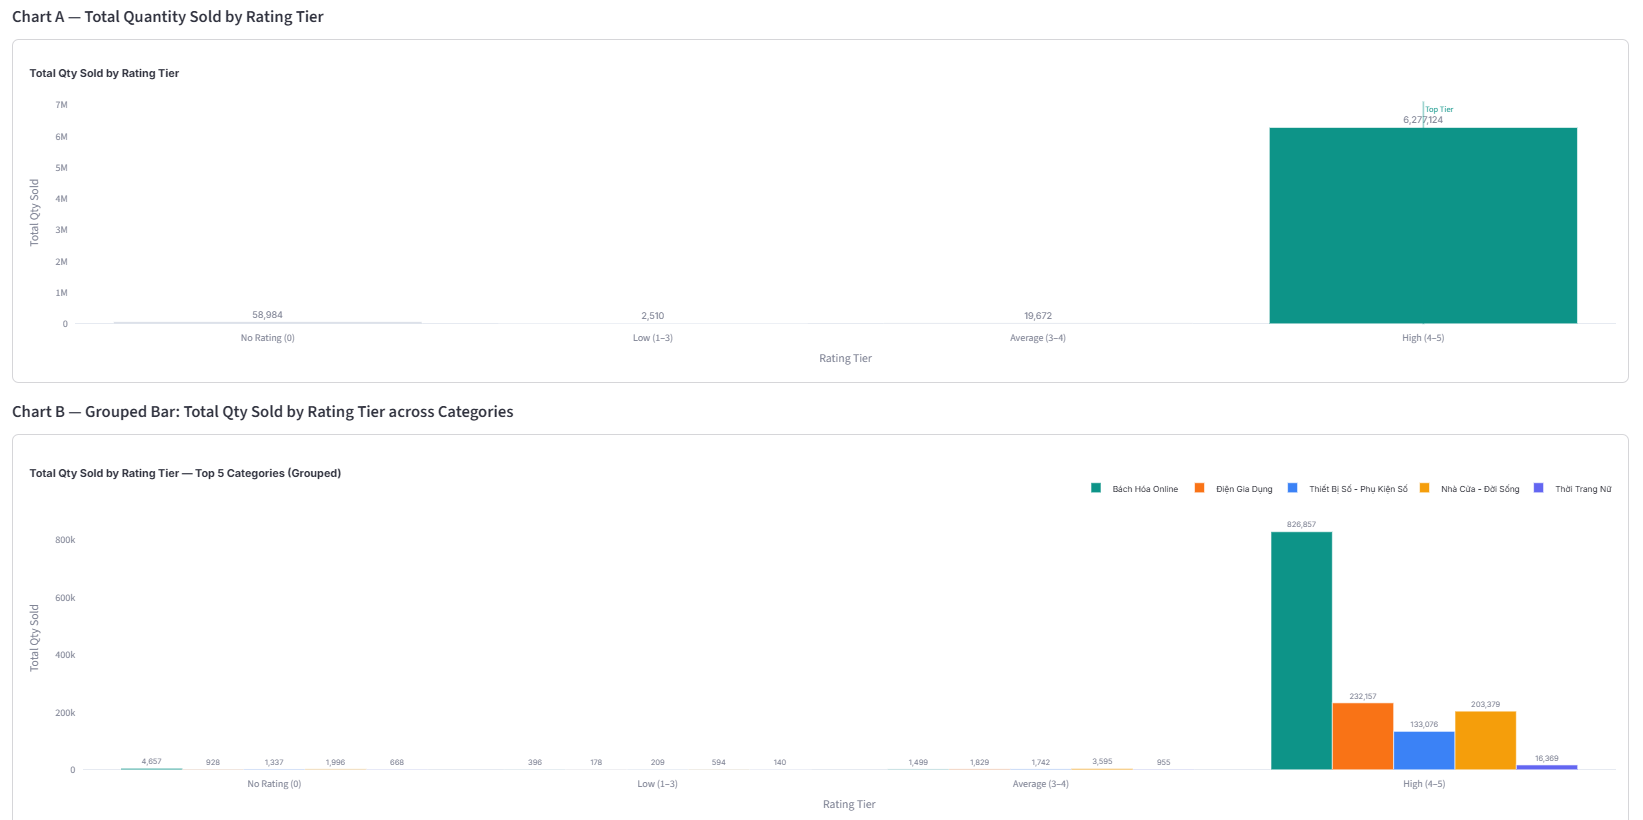
\includegraphics[width=0.95\textwidth]{graphics/trust_pic1.png} 
    \caption{Phân tích đa chiều về tác động của điểm đánh giá trung bình đến doanh số bán hàng trên nền tảng Tiki.}
    \label{fig:tiki_rating_sales}
\end{figure}

\textbf{Nhận xét và kết luận:}
\begin{itemize}
    \item \textbf{Ngưỡng tin cậy và Sự đứt gãy doanh số:} Biểu đồ (a) cho thấy sự tăng trưởng đột biến về doanh số khi sản phẩm đạt mức đánh giá \textbf{Cao (4-5 sao)}. Ngược lại, nhóm \textit{No Rating (0)} ghi nhận giá trị tiệm cận 0, minh chứng cho rào cản niềm tin cực lớn: nếu không có đánh giá, sản phẩm gần như không có cơ hội chuyển đổi.
    \item \textbf{Sức mạnh của nhãn chứng thực (Badge Effect):} Biểu đồ (b) làm nổi bật vai trò của nhãn Best Seller như một biến số thúc đẩy doanh số. Khi sản phẩm đã vượt qua ngưỡng tin cậy 4-5 sao, việc sở hữu nhãn Best Seller giúp doanh số trung bình tăng vọt gấp gần 3 lần so với hàng thông thường. Điều này cho thấy khách hàng chỉ ưu tiên hiệu ứng đám đông khi rủi ro về chất lượng đã được loại bỏ bởi điểm đánh giá cao.
    \item \textbf{Kết luận:} Nhãn Best Seller không phải là phép màu cho mọi sản phẩm, mà là một cú hit cực mạnh chỉ phát huy tác dụng khi đi kèm với Rating tốt. 
    \item \textbf{Hành động chiến lược:} Doanh nghiệp cần tập trung nguồn lực đẩy các sản phẩm cận biên (3.8 - 3.9 sao) vượt ngưỡng 4.0 sao để nhãn Best Seller có thể phát huy tối đa sức mạnh thúc đẩy doanh thu bùng nổ.
\end{itemize}

\subsubsection{Mục tiêu 8}

\textbf{Phương pháp trực quan:}
\begin{itemize}
    \item \textbf{Nguyên lý Stratification (Phân tầng):} Sử dụng biểu đồ \textit{Stratified Box Plot} để bóc tách dữ liệu thành 4 tầng uy tín riêng biệt. Cách tiếp cận này không chỉ hiển thị mức giá trung tâm mà còn phơi bày độ biến động (\textit{IQR}) và rủi ro thị trường trong từng nhóm người bán.
    \item \textbf{Nguyên lý Connection (Kết nối):} Sử dụng biểu đồ đường (\textit{Trendline}) kết nối các giá trị trung vị giữa các cột. Phương pháp này dẫn dắt ánh nhìn theo một lộ trình tuyến tính, minh chứng cho quy luật tăng trưởng giá trị dựa trên lòng tin (\textit{Trust-based Pricing}).
    \item \textbf{Tối ưu hóa Data-Ink Ratio:} Loại bỏ các đường lưới không cần thiết và sử dụng các điểm chấm (\textit{Outliers}) để biểu thị những mặt hàng có giá trị cực cao, giúp giữ cho biểu đồ sạch sẽ nhưng vẫn đầy đủ thông tin về các trường hợp đặc biệt.
\end{itemize}

\textbf{Kết quả trực quan hóa:}

\begin{figure}[H]
    \centering
    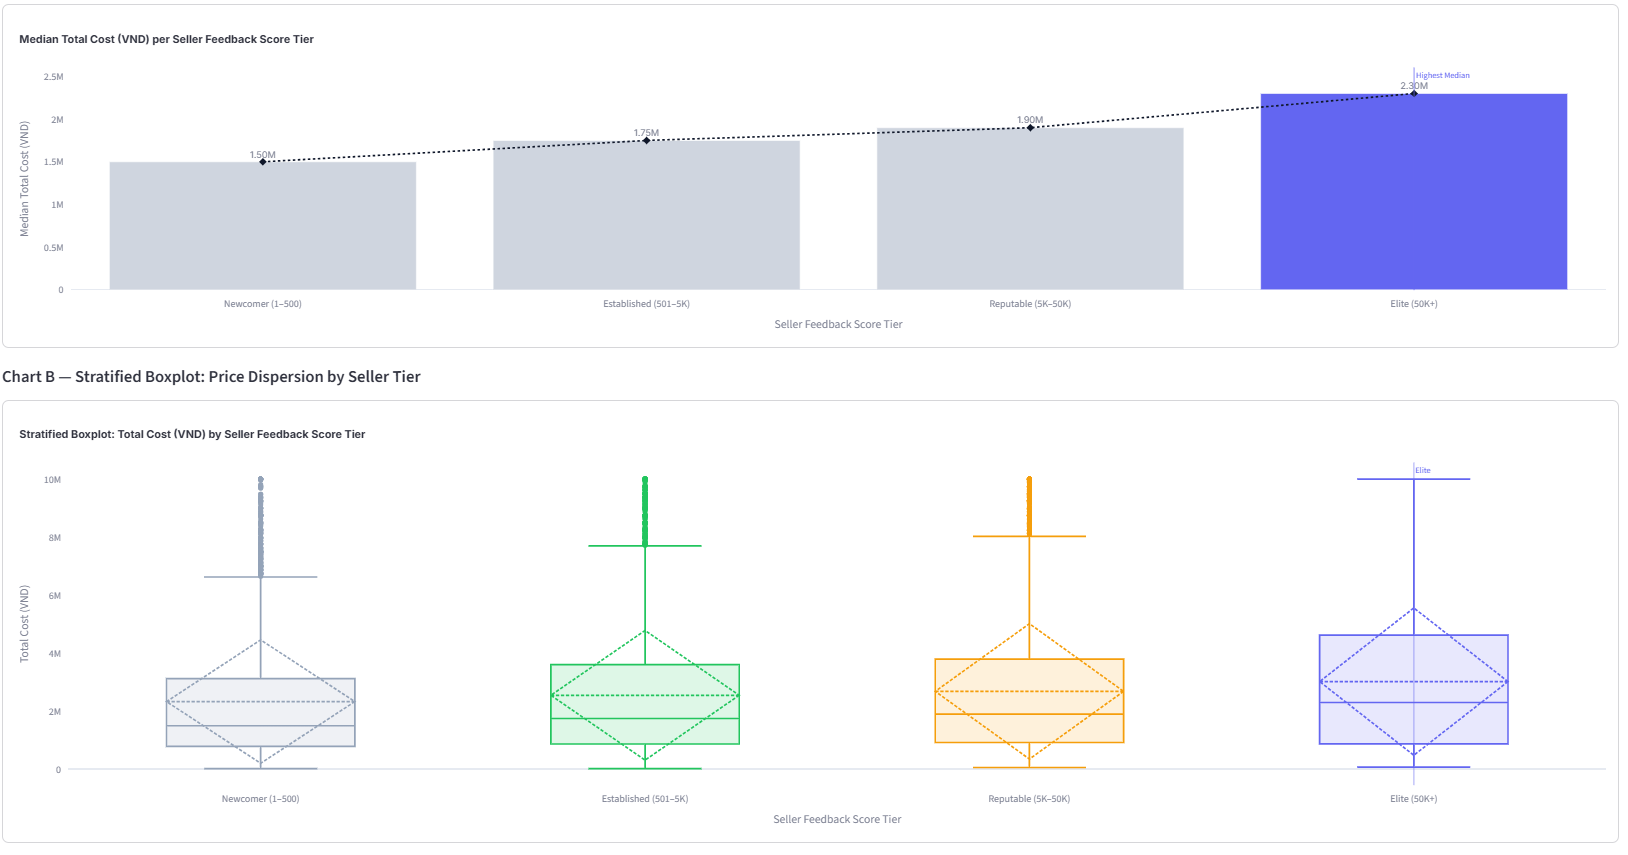
\includegraphics[width=0.95\textwidth]{graphics/trust_pic2.png} 
    \caption{Biểu đồ phân tầng uy tín người bán và sự phân tán giá niêm yết trên nền tảng eBay.}
    \label{fig:ebay_objective_8}
\end{figure}

\textbf{Nhận xét và kết luận:}
\begin{itemize}
    \item \textbf{Tương quan thuận giữa uy tín và giá trị:} Dữ liệu chỉ ra một xu hướng nhất quán: khi cấp độ uy tín tăng lên, mức giá niêm yết trung vị cũng tăng theo. Nhóm \textbf{Elite (50K+)} ghi nhận mức giá trung bình cao nhất, trong khi nhóm \textbf{Newcomer} duy trì mức giá thấp nhất để đảm bảo tính cạnh tranh.
    \item \textbf{Độ ổn định và Rủi ro (IQR):} Chỉ số \textit{IQR} ở tầng \textbf{Elite} cho thấy sự tập trung giá hẹp, phản ánh chiến lược định giá chuyên nghiệp. Ngược lại, nhóm \textbf{Newcomer} có độ phân tán giá rộng, minh chứng cho sự hỗn loạn trong giai đoạn đầu dò xét thị trường và sự không đồng nhất về chất lượng sản phẩm.
    \item \textbf{Kết luận:} Trên eBay, uy tín người bán là một loại "tài sản thương hiệu" cho phép áp dụng mức giá cao cấp (\textit{Premium Price}). Người mua sẵn sàng trả phí cao hơn để đổi lấy sự cam kết về chất lượng từ các tầng uy tín cao.
    \item \textbf{Hành động chiến lược:} Dashboard khuyến nghị người bán mới nên chấp nhận mức biên lợi nhuận thấp để tích lũy điểm phản hồi (\textit{feedback score}). Đối với nhà quản trị sàn, cần có chính sách kiểm soát chặt chẽ nhóm \textit{Newcomer} do độ biến động giá cao, tiềm ẩn rủi ro về trải nghiệm người dùng.
\end{itemize}

\subsection{Interactive Dashboard}

\subsubsection{Thiết kế Dashboard}

Dashboard được xây dựng bằng [Streamlit/Dash] với cấu trúc gồm 3 tab chính:

\textbf{Tab 1: Tổng quan (Overview)}
\begin{itemize}
    \item Các chỉ số KPI chính
    \item Biểu đồ tổng quan về dữ liệu
    \item Thống kê mô tả cơ bản
\end{itemize}

\textbf{Tab 2: Phân tích chi tiết (Detailed Analysis)}
\begin{itemize}
    \item Phân tích theo từng mục tiêu
    \item Các biểu đồ tương tác
    \item Bộ lọc và selector
\end{itemize}

\textbf{Tab 3: So sánh và Tổng kết (Comparison \& Summary)}
\begin{itemize}
    \item So sánh giữa các nhóm/danh mục
    \item Kết luận tổng hợp
    \item Khuyến nghị
\end{itemize}

\subsubsection{Các tính năng tương tác}

\begin{itemize}
    \item \textbf{Filter:} Lọc theo danh mục, khoảng giá, đánh giá
    \item \textbf{Selector:} Chọn khoảng thời gian, cửa hàng
    \item \textbf{Hover:} Hiển thị thông tin chi tiết khi di chuột
    \item \textbf{Zoom:} Phóng to/thu nhỏ biểu đồ
    \item \textbf{Download:} Tải xuống dữ liệu và biểu đồ
\end{itemize}

\subsubsection{Ảnh chụp Dashboard}

% \begin{figure}[H]
%     \centering
%     \includegraphics[width=\textwidth]{graphics/dashboard_overview.png}
%     \caption{Giao diện Dashboard - Tab Tổng quan}
%     \label{fig:dashboard_1}
% \end{figure}

% \begin{figure}[H]
%     \centering
%     \includegraphics[width=\textwidth]{graphics/dashboard_analysis.png}
%     \caption{Giao diện Dashboard - Tab Phân tích chi tiết}
%     \label{fig:dashboard_2}
% \end{figure}

\subsection{Ứng dụng Machine Learning (Điểm cộng)}

\subsubsection{Mô hình sử dụng}

\textbf{Bài toán:} Phân loại nhị phân (Binary Classification) — dự đoán liệu một sản phẩm trên Tiki có khả năng đạt trạng thái \textbf{Best Seller} hay không, dựa trên các đặc trưng về giá, tỷ lệ giảm giá, đánh giá và thông tin danh mục/thương hiệu.

\textbf{Mô hình:} XGBoost Classifier (\textit{eXtreme Gradient Boosting}) với xử lý mất cân bằng lớp bằng tham số \texttt{scale\_pos\_weight}.

\textbf{Đặc trưng đầu vào (Features):}
\begin{itemize}
    \item \textbf{price} — Giá bán hiện tại (VND)
    \item \textbf{original\_price} — Giá gốc trước khi giảm (VND)
    \item \textbf{discount\_rate} — Tỷ lệ giảm giá (\%)
    \item \textbf{rating\_average} — Điểm đánh giá trung bình (0–5)
    \item \textbf{Price\_Gap} — Khoảng cách giá = original\_price $-$ price (feature engineering)
    \item \textbf{brand\_freq} — Tần suất xuất hiện của thương hiệu trong dataset (Frequency Encoding)
    \item \textbf{category\_freq} — Tần suất xuất hiện của danh mục trong dataset (Frequency Encoding)
\end{itemize}

\textbf{Siêu tham số (Hyperparameters):}
\begin{itemize}
    \item \texttt{n\_estimators=350}, \texttt{max\_depth=5}, \texttt{learning\_rate=0.05}
    \item \texttt{subsample=0.9}, \texttt{colsample\_bytree=0.9}
    \item \texttt{scale\_pos\_weight} $\approx$ 3.1 (tỷ lệ negative/positive để xử lý class imbalance)
\end{itemize}

\subsubsection{Kết quả và trực quan hóa}

\textbf{Tập dữ liệu huấn luyện/kiểm tra:} 80\% train / 20\% test (stratified), test set gồm 2.000 mẫu (1.513 Non Best Seller / 487 Best Seller).

\begin{table}[H]
    \centering
    \caption{Kết quả phân loại mô hình XGBoost trên tập kiểm tra}
    \begin{tabular}{|l|c|c|c|c|}
        \hline
        \textbf{Class} & \textbf{Precision} & \textbf{Recall} & \textbf{F1-Score} & \textbf{Support} \\
        \hline
        Non Best Seller (0) & 0.939 & 0.831 & 0.882 & 1,513 \\
        \hline
        Best Seller (1)     & 0.614 & 0.832 & 0.706 &   487 \\
        \hline
        \textbf{Accuracy}   & \multicolumn{4}{c|}{\textbf{83.15\%}} \\
        \hline
        Macro Avg           & 0.776 & 0.832 & 0.794 & 2,000 \\
        \hline
        Weighted Avg        & 0.860 & 0.832 & 0.839 & 2,000 \\
        \hline
    \end{tabular}
    \label{tab:ml_classification_report}
\end{table}

\textbf{ROC-AUC:} 0.915 (xếp loại Excellent — mô hình phân biệt đúng cặp Best Seller / Non Best Seller trong 91.5\% trường hợp).

\textbf{Kết quả trực quan hóa:}

\begin{figure}[H]
    \centering
    \begin{minipage}{0.48\textwidth}
        \centering
        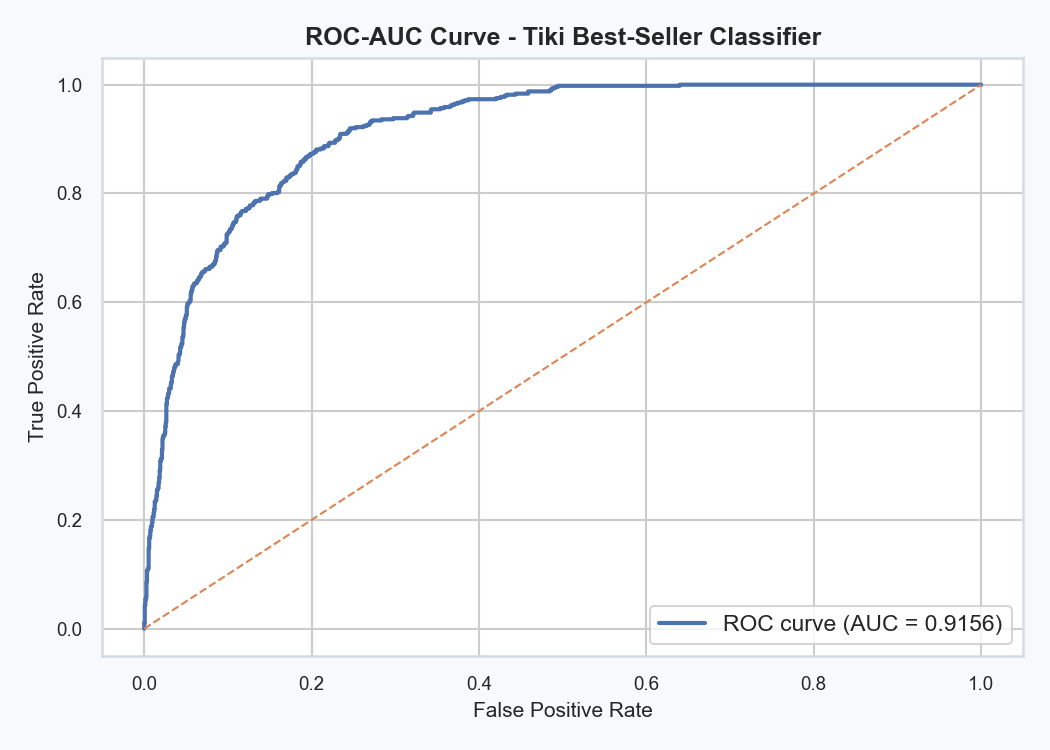
\includegraphics[width=\textwidth]{../models/roc_auc_curve.png}
        \caption{Đường cong ROC-AUC của mô hình XGBoost phân loại Best Seller Tiki.}
        \label{fig:ml_roc_auc}
    \end{minipage}
    \hfill
    \begin{minipage}{0.48\textwidth}
        \centering
        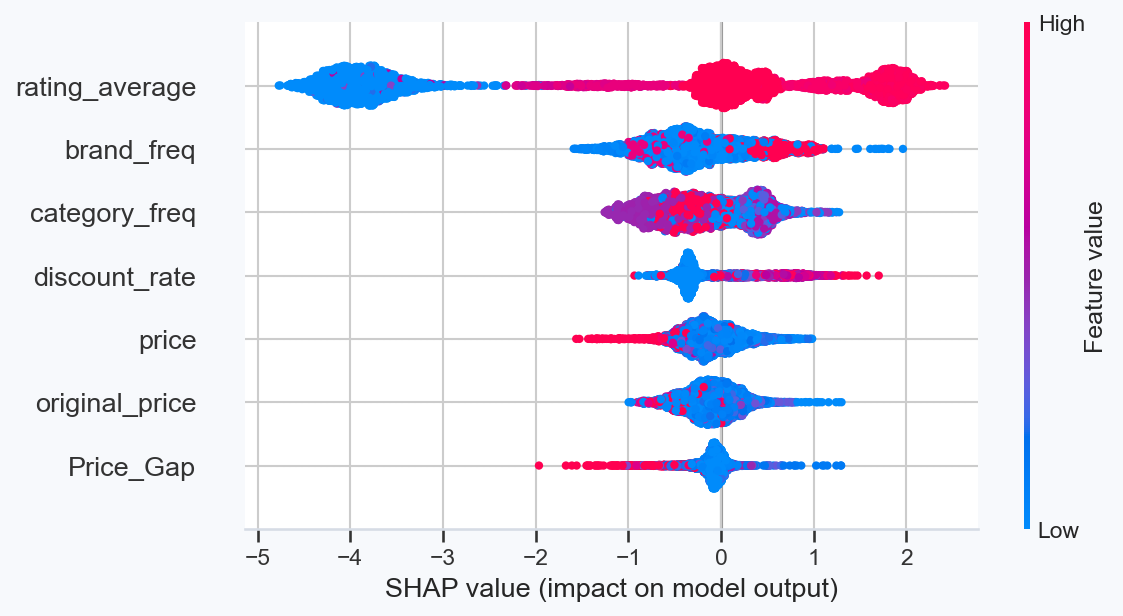
\includegraphics[width=\textwidth]{../models/shap_summary.png}
        \caption{Biểu đồ SHAP thể hiện mức độ ảnh hưởng của từng đặc trưng đến dự đoán Best Seller.}
        \label{fig:ml_shap}
    \end{minipage}
\end{figure}

\textbf{Đánh giá mô hình:}
\begin{itemize}
    \item \textbf{ROC-AUC = 0.915:} Mô hình phân biệt rất tốt giữa hai lớp, đặc biệt khi xét đến tỷ lệ mất cân bằng lớp (Best Seller chỉ chiếm \~{}24\%).
    \item \textbf{Recall (Best Seller) = 83.2\%:} Mô hình tìm được 405/487 sản phẩm Best Seller thực tế, chỉ bỏ sót 82 trường hợp.
    \item \textbf{Precision (Best Seller) = 61.4\%:} Một phần sản phẩm được dự đoán là Best Seller thực tế không phải (255 False Positives), phản ánh sự đánh đổi khi ưu tiên Recall để không bỏ sót.
\end{itemize}

\textbf{Ý nghĩa phân tích:} Thông qua giá trị SHAP, mô hình xác nhận \textbf{rating\_average} và \textbf{discount\_rate} là hai yếu tố ảnh hưởng lớn nhất đến khả năng đạt Best Seller — nhất quán với kết quả phân tích định tính ở Mục tiêu 2 và 7. Điều này gợi ý rằng chiến lược tối ưu cho người bán Tiki là kết hợp đồng thời giữa mức giảm giá 20–50\% và duy trì chất lượng sản phẩm để đạt rating $\geq$ 4.0 sao.

\clearpage
